% A small feed-forward network glyph for Figure 2: three inputs, two hidden layers of
% five, five outputs (the classes). Compile with
%   pdflatex -jobname=network_black network.tex
%   pdflatex -jobname=network_blue "\def\netcolour{0077BB}% A small feed-forward network glyph for Figure 2: three inputs, two hidden layers of
% five, five outputs (the classes). Compile with
%   pdflatex -jobname=network_black network.tex
%   pdflatex -jobname=network_blue "\def\netcolour{0077BB}% A small feed-forward network glyph for Figure 2: three inputs, two hidden layers of
% five, five outputs (the classes). Compile with
%   pdflatex -jobname=network_black network.tex
%   pdflatex -jobname=network_blue "\def\netcolour{0077BB}% A small feed-forward network glyph for Figure 2: three inputs, two hidden layers of
% five, five outputs (the classes). Compile with
%   pdflatex -jobname=network_black network.tex
%   pdflatex -jobname=network_blue "\def\netcolour{0077BB}\input{network.tex}"
\documentclass[border=2pt,tikz]{standalone}
\usepackage{xcolor}
\providecommand{\netcolour}{000000}
\definecolor{netcol}{HTML}{\netcolour}
\begin{document}
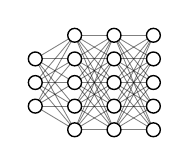
\begin{tikzpicture}[x=0.5cm,y=0.3cm,
  neuron/.style={circle,draw=netcol,fill=white,line width=0.5pt,minimum size=5pt,inner sep=0pt},
  link/.style={draw=netcol,line width=0.3pt,opacity=0.5}]
  % links first, so that the neurons cover their ends
  \foreach \l/\n/\m in {0/3/5,1/5/5,2/5/5} {
    \pgfmathtruncatemacro{\lnext}{\l+1}
    \foreach \i in {1,...,\n} {
      \foreach \j in {1,...,\m} {
        \draw[link] (\l,{\i-(\n+1)/2}) -- (\lnext,{\j-(\m+1)/2});
      }
    }
  }
  \foreach \l/\n in {0/3,1/5,2/5,3/5} {
    \foreach \i in {1,...,\n} {
      \node[neuron] at (\l,{\i-(\n+1)/2}) {};
    }
  }
\end{tikzpicture}
\end{document}
"
\documentclass[border=2pt,tikz]{standalone}
\usepackage{xcolor}
\providecommand{\netcolour}{000000}
\definecolor{netcol}{HTML}{\netcolour}
\begin{document}
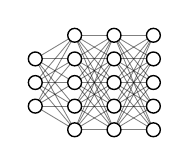
\begin{tikzpicture}[x=0.5cm,y=0.3cm,
  neuron/.style={circle,draw=netcol,fill=white,line width=0.5pt,minimum size=5pt,inner sep=0pt},
  link/.style={draw=netcol,line width=0.3pt,opacity=0.5}]
  % links first, so that the neurons cover their ends
  \foreach \l/\n/\m in {0/3/5,1/5/5,2/5/5} {
    \pgfmathtruncatemacro{\lnext}{\l+1}
    \foreach \i in {1,...,\n} {
      \foreach \j in {1,...,\m} {
        \draw[link] (\l,{\i-(\n+1)/2}) -- (\lnext,{\j-(\m+1)/2});
      }
    }
  }
  \foreach \l/\n in {0/3,1/5,2/5,3/5} {
    \foreach \i in {1,...,\n} {
      \node[neuron] at (\l,{\i-(\n+1)/2}) {};
    }
  }
\end{tikzpicture}
\end{document}
"
\documentclass[border=2pt,tikz]{standalone}
\usepackage{xcolor}
\providecommand{\netcolour}{000000}
\definecolor{netcol}{HTML}{\netcolour}
\begin{document}
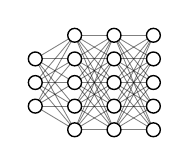
\begin{tikzpicture}[x=0.5cm,y=0.3cm,
  neuron/.style={circle,draw=netcol,fill=white,line width=0.5pt,minimum size=5pt,inner sep=0pt},
  link/.style={draw=netcol,line width=0.3pt,opacity=0.5}]
  % links first, so that the neurons cover their ends
  \foreach \l/\n/\m in {0/3/5,1/5/5,2/5/5} {
    \pgfmathtruncatemacro{\lnext}{\l+1}
    \foreach \i in {1,...,\n} {
      \foreach \j in {1,...,\m} {
        \draw[link] (\l,{\i-(\n+1)/2}) -- (\lnext,{\j-(\m+1)/2});
      }
    }
  }
  \foreach \l/\n in {0/3,1/5,2/5,3/5} {
    \foreach \i in {1,...,\n} {
      \node[neuron] at (\l,{\i-(\n+1)/2}) {};
    }
  }
\end{tikzpicture}
\end{document}
"
\documentclass[border=2pt,tikz]{standalone}
\usepackage{xcolor}
\providecommand{\netcolour}{000000}
\definecolor{netcol}{HTML}{\netcolour}
\begin{document}
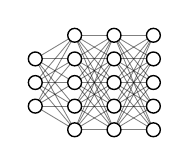
\begin{tikzpicture}[x=0.5cm,y=0.3cm,
  neuron/.style={circle,draw=netcol,fill=white,line width=0.5pt,minimum size=5pt,inner sep=0pt},
  link/.style={draw=netcol,line width=0.3pt,opacity=0.5}]
  % links first, so that the neurons cover their ends
  \foreach \l/\n/\m in {0/3/5,1/5/5,2/5/5} {
    \pgfmathtruncatemacro{\lnext}{\l+1}
    \foreach \i in {1,...,\n} {
      \foreach \j in {1,...,\m} {
        \draw[link] (\l,{\i-(\n+1)/2}) -- (\lnext,{\j-(\m+1)/2});
      }
    }
  }
  \foreach \l/\n in {0/3,1/5,2/5,3/5} {
    \foreach \i in {1,...,\n} {
      \node[neuron] at (\l,{\i-(\n+1)/2}) {};
    }
  }
\end{tikzpicture}
\end{document}
